\documentclass{article}

\usepackage[spanish]{babel}
\usepackage{graphicx} % Required for the inclusion of images
\usepackage{amsmath} % Required for some math elements 
\usepackage{hyperref}
\usepackage{amsmath}
\usepackage{listings}
\usepackage{xcolor}
\usepackage{courier}
\usepackage[margin=1in]{geometry}
\usepackage{changepage}
\usepackage{titlesec}
\usepackage{wrapfig}
\usepackage[version=4]{mhchem}
\usepackage{multirow}
\usepackage{siunitx}
\usepackage{ragged2e}
\usepackage{adjustbox}
\usepackage{caption}

\definecolor{codegreen}{rgb}{0,0.6,0}
\definecolor{codegray}{rgb}{0.5,0.5,0.5}
\definecolor{codepurple}{rgb}{0.58,0,0.82}
\definecolor{backcolour}{rgb}{0.95,0.95,0.92}

\lstdefinestyle{mystyle}{
    backgroundcolor=\color{backcolour},   
    commentstyle=\color{codegreen},
    keywordstyle=\color{magenta},
    numberstyle=\tiny\color{codegray},
    stringstyle=\color{codepurple},
    basicstyle=\ttfamily\footnotesize,
    breakatwhitespace=false,         
    captionpos=b,                    
    keepspaces=true,                 
    numbers=left,                    
    numbersep=5pt,                  
    showspaces=false,                
    showstringspaces=false,
    showtabs=false,                  
    tabsize=2
}
\lstset{language=Python, 
        basicstyle=\ttfamily\small, 
        keywordstyle=\color{keywords},
        commentstyle=\color{comments},
        stringstyle=\color{red},
        showstringspaces=false,
        identifierstyle=\color{codepurple},
        keywords=[2]{pow},
        keywordstyle=[2]{\color{orange}},
}

\lstset{style=mystyle}
\setlength\parindent{0pt}
\renewcommand{\labelenumi}{\alph{enumi}.}

\title{\textbf{Análisis del movimiento \\ de cargas bajo el efecto \\ de campos magnéticos}}

\author{Víctor Mira Ramírez}

\date{\today}

\begin{document}

\maketitle

\begin{center}
\begin{tabular}{l r}

Profesor: & Carlos Untiedt Lecuona\\
Lugar: & Universidad de Alicante
\end{tabular}
\end{center}

\tableofcontents

\begin{abstract}
    \noindent En esta práctica de ordenador vamos a estudiar mediante el
    uso de programas, en lenguaje python, el movimiento de cargas en
    campos electromagnéticos. Para ello resolveremos las ecuaciones
    de movimiento mediante el uso de algoritmos. Analizaremos
    distintos instrumentos basados en la acción de campos
    electromagnéticos sobre partículas cargadas como el espectrómetro
    de masas, el selector de velocidades o el ciclotrón. 
    \\ \\La primera parte de la práctica la dedicaremos a la obtención de las
    ecuaciones de movimiento de una partícula cargada en un campo
    electromagnético. En la segunda parte resolveremos las
    ecuaciones de movimiento y analizaremos los resultados numéricos
    obtenidos para cada caso.
\end{abstract}
    
\newpage
    
\section{Espectrómetro de Masas}
    \subsection{Funcionamiento}
    El siguiente diagrama muestra un ciclotrón y las fuerzas que actúan sobre él. Podemos observar una posible trayectoria que una partícula seguiría en él en rojo.
    \\ \\ La diferencia de potencial esta representada por las dos líneas negras paralelas al eje x, que distan una distancia h entre sí. Llamaremos región I a la zona que hay entre ambas. Esta diferencia de potencial solo dejará pasar a las partículas cargadas que vayan a una velocidad concreta que se desee, para que así giren una vez entren en la siguiente región.
    \\ \\ En esta otra región, un campo magnético se sitúa justo sobre la placa de menor potencial, perpendicular a la trayectoria de las partículas y formando lo que llamaremos región II. Esta hará que las cargas en movimiento giren hasta alcanzar una distancia D que las separe del origen.
    
    \begin{figure}[h]
    \centering
    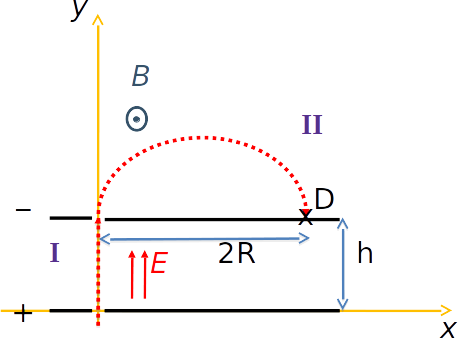
\includegraphics[width=.6\textwidth]{Fotos/espectrometro.png}
    \end{figure}
    
    En resumen, partículas cargadas procedentes de una fuente que suponemos inicialmente en reposo son aceleradas en la región I mediante un campo eléctrico E, que posteriormente penetran en una región II con un campo magnético B perpendicular que los desvía. \\\\ Vamos a simular la trayectoria de estas partículas cargadas y calcular la distancia D que habrá entre el origen y el punto en el que incidirán.
    
    \subsection{Pruebas con muestras de iones}
    Mediante el uso del script de python, simularemos el paso por un espectrómetro de masas con campos electromagnéticos de intensidad aleatoria en función de una semilla que en este caso es mi DNI. El campo magnético podrá variar entre $2\cdot10^{-2}T$ y $1\cdot10^{-1}T$ y el campo eléctrico entre $10 V$ y $30 V$.
    
    \clearpage
    
    \subsubsection{Resultados}
    
    \begin{figure}[h]
        \hspace*{-0.6cm}
        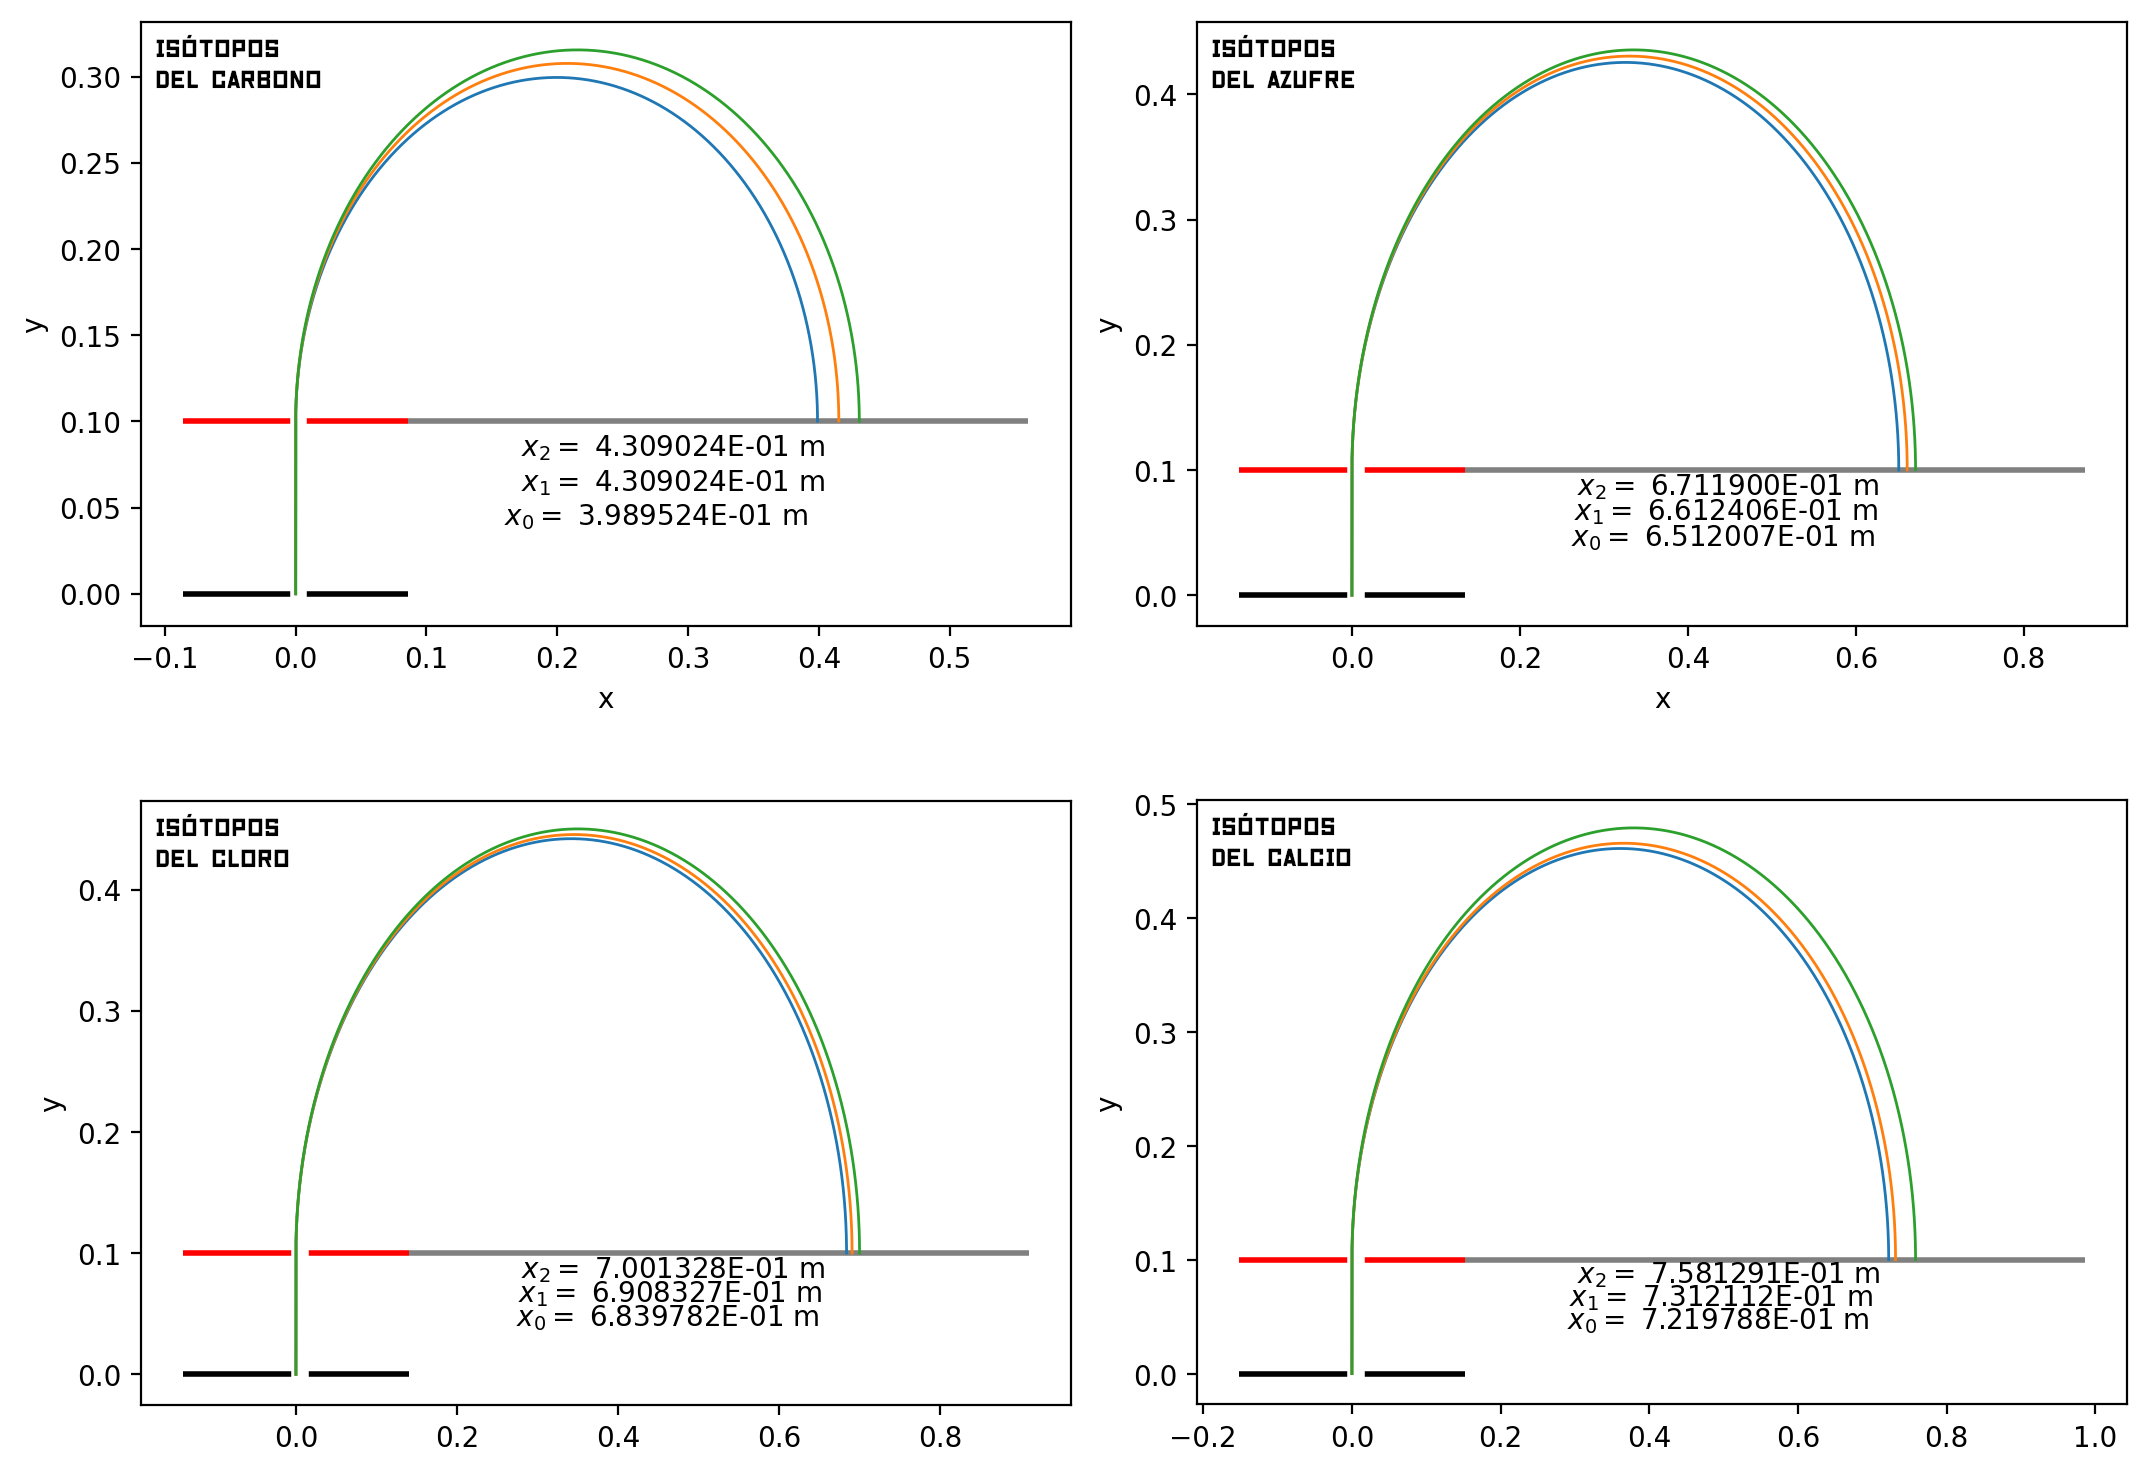
\includegraphics[width=1\textwidth]{Fotos/isotopos.png}
        \hspace*{-2cm}
    \end{figure}

\hfill

\begin{table}[h!]
\setlength{\tabcolsep}{3pt}
    \renewcommand{\arraystretch}{1.5}
\hspace*{-1.2cm}
\fontsize{6.5}{9}\selectfont
\centering
\begin{tabular}{cccccllccccc}
\cline{1-5} \cline{8-12}
\multicolumn{1}{|c|}{$B=0.012T$} & \multicolumn{2}{c|}{\normalsize\multirow{3}{*}{Cálculo Analítico}} & \multicolumn{2}{c|}{\multirow{3}{*}{\normalsize Cálculo Numérico}} &  & \multicolumn{1}{l|}{} & \multicolumn{1}{c|}{$B=0.012T$} & \multicolumn{2}{c|}{\multirow{3}{*}{\normalsize Cálculo Analítico}} & \multicolumn{2}{c|}{\multirow{3}{*}{\normalsize Cálculo Numérico}} \\
\multicolumn{1}{|c|}{$\Delta V = 23 V$} & \multicolumn{2}{c|}{} & \multicolumn{2}{c|}{} &  & \multicolumn{1}{l|}{} & \multicolumn{1}{c|}{$\Delta V = 23 V$} & \multicolumn{2}{c|}{} & \multicolumn{2}{c|}{} \\
\multicolumn{1}{|c|}{$h=0.1cm$} & \multicolumn{2}{c|}{} & \multicolumn{2}{c|}{} &  & \multicolumn{1}{l|}{} & \multicolumn{1}{c|}{$h=0.1cm$} & \multicolumn{2}{c|}{} & \multicolumn{2}{c|}{} \\ \cline{1-5} \cline{8-12}
\multicolumn{1}{|c|}{\small Elemento} & \multicolumn{1}{c|}{\small $t_a(s)$} & \multicolumn{1}{c|}{\small $D_a(m)$} & \multicolumn{1}{c|}{\small $t_n(s)$} & \multicolumn{1}{c|}{\small $D_n(m)$} &  & \multicolumn{1}{l|}{} & \multicolumn{1}{c|}{\small Elemento} & \multicolumn{1}{c|}{\small $t_a(s)$} & \multicolumn{1}{c|}{\small $D_a(m)$} & \multicolumn{1}{c|}{\small $t_n(s)$} & \multicolumn{1}{c|}{\small $D_n(m)$} \\ \cline{1-5} \cline{8-12}

\multicolumn{1}{|c|}{$x_1= \ce{^{12}C+}$} & \multicolumn{1}{c|}{$4.3017 \cdot 10^{-5}$} & \multicolumn{1}{c|}{$3.989526 \cdot 10^{-1}$} & \multicolumn{1}{c|}{$4.3024 \cdot 10^{-5}$} & \multicolumn{1}{c|}{$3.989524 \cdot 10^{-1}$} &  & \multicolumn{1}{l|}{} & \multicolumn{1}{c|}{$x_1= \ce{^{32}S+}$} & \multicolumn{1}{c|}{$1.0387 \cdot 10^{-4}$} & \multicolumn{1}{c|}{$3.256004 \cdot 10^{-1}$} & \multicolumn{1}{c|}{$1.0388 \cdot 10^{-4}$} & \multicolumn{1}{c|}{$ 6.512007\cdot 10^{-1}$} \\ \cline{1-5} \cline{8-12} 
\multicolumn{1}{|c|}{$x_2 = \ce{^{13}C+}$} & \multicolumn{1}{c|}{$4.6158\cdot 10^{-5}$} & \multicolumn{1}{c|}{$4.152350\cdot 10^{-1}$} & \multicolumn{1}{c|}{$ 4.6159\cdot 10^{-5}$} & \multicolumn{1}{c|}{$4.152348 \cdot 10^{-1}$} &  & \multicolumn{1}{l|}{} & \multicolumn{1}{c|}{$x_2 = \ce{^{33}S+}$} & \multicolumn{1}{c|}{$1.0683 \cdot 10^{-4}$} & \multicolumn{1}{c|}{$ 3.306204\cdot 10^{-4}$} & \multicolumn{1}{c|}{$1.0684 \cdot 10^{-4}$} & \multicolumn{1}{c|}{$6.612406 \cdot 10^{-1}$} \\ \cline{1-5} \cline{8-12} 
\multicolumn{1}{|c|}{$x_3 = \ce{^{14}C+}$} & \multicolumn{1}{c|}{$4.9283\cdot 10^{-5}$} & \multicolumn{1}{c|}{$4.309026\cdot 10^{-1}$} & \multicolumn{1}{c|}{$ 4.9294\cdot 10^{-5}$} & \multicolumn{1}{c|}{$4.309024 \cdot 10^{-1}$} &  & \multicolumn{1}{l|}{} & \multicolumn{1}{c|}{$x_3 = \ce{^{34}S+}$} & \multicolumn{1}{c|}{$1.0980 \cdot 10^{-4}$} & \multicolumn{1}{c|}{$ 6.711903\cdot 10^{-1}$} & \multicolumn{1}{c|}{$1.0981 \cdot 10^{-4}$} & \multicolumn{1}{c|}{$6.711900 \cdot 10^{-1}$} \\ \cline{1-5} \cline{8-12} 
\multicolumn{1}{l}{} & \multicolumn{1}{l}{} & \multicolumn{1}{l}{} & \multicolumn{1}{l}{} & \multicolumn{1}{l}{} &  &  & \multicolumn{1}{l}{} & \multicolumn{1}{l}{} & \multicolumn{1}{l}{} & \multicolumn{1}{l}{} & \multicolumn{1}{l}{} \\ \cline{1-5} \cline{8-12} 
\multicolumn{1}{|c|}{$B=0.012T$} & \multicolumn{2}{c|}{\multirow{3}{*}{\normalsize Cálculo Analítico}} & \multicolumn{2}{c|}{\multirow{3}{*}{\normalsize Cálculo Numérico}} & \multicolumn{1}{c}{} & \multicolumn{1}{l|}{} & \multicolumn{1}{c|}{$B=0.012T$} & \multicolumn{2}{c|}{\multirow{3}{*}{\normalsize Cálculo Analítico}} & \multicolumn{2}{c|}{\multirow{3}{*}{\normalsize Cálculo Numérico}} \\
\multicolumn{1}{|c|}{$\Delta V = 23 V$} & \multicolumn{2}{c|}{} & \multicolumn{2}{c|}{} & \multicolumn{1}{c}{} & \multicolumn{1}{c|}{} & \multicolumn{1}{c|}{$\Delta V = 23 V$} & \multicolumn{2}{c|}{} & \multicolumn{2}{c|}{} \\
\multicolumn{1}{|c|}{$h=0.1cm$} & \multicolumn{2}{c|}{} & \multicolumn{2}{c|}{} & \multicolumn{1}{c}{} & \multicolumn{1}{c|}{} & \multicolumn{1}{c|}{$h=0.1cm$} & \multicolumn{2}{c|}{} & \multicolumn{2}{c|}{} \\ \cline{1-5} \cline{8-12}
\multicolumn{1}{|c|}{\small Elemento} & \multicolumn{1}{c|}{\small $t_a(s)$} & \multicolumn{1}{c|}{\small $D_a(m)$} & \multicolumn{1}{c|}{\small $t_n(s)$} & \multicolumn{1}{c|}{\small $D_n(m)$} &  & \multicolumn{1}{l|}{} & \multicolumn{1}{c|}{\small Elemento} & \multicolumn{1}{c|}{\small $t_a(s)$} & \multicolumn{1}{c|}{\small $D_a(m)$} & \multicolumn{1}{c|}{\small $t_n(s)$} & \multicolumn{1}{c|}{\small $D_n(m)$} \\ \cline{1-5} \cline{8-12} 
\multicolumn{1}{|c|}{$x_1= \ce{^{35}Cl+}$} & \multicolumn{1}{c|}{$1.1369\cdot 10^{-4}$} & \multicolumn{1}{c|}{$6.839784\cdot 10^{-1}$} & \multicolumn{1}{c|}{$1.1369\cdot 10^{-4}$} & \multicolumn{1}{c|}{$6.839782 \cdot 10^{-1}$} &  & \multicolumn{1}{l|}{} & \multicolumn{1}{c|}{$x_1= \ce{^{39}Ca+}$} & \multicolumn{1}{c|}{$1.2563\cdot 10^{-4}$} & \multicolumn{1}{c|}{$7.219788\cdot10^{-1}$} & \multicolumn{1}{c|}{$1.2563\cdot 10^{-4}$} & \multicolumn{1}{c|}{$7.219788\cdot 10^{-1}$} \\ \cline{1-5} \cline{8-12} 
\multicolumn{1}{|c|}{$x_2 = \ce{^{36}Cl+}$} & \multicolumn{1}{c|}{$1.1580 \cdot 10^{-4}$} & \multicolumn{1}{c|}{$6.908328\cdot 10^{-1}$} & \multicolumn{1}{c|}{$1.1581 \cdot 10^{-4}$} & \multicolumn{1}{c|}{$6.908327 \cdot 10^{-1}$} &  & \multicolumn{1}{l|}{} & \multicolumn{1}{c|}{$x_2 = \ce{^{40}Ca+}$} & \multicolumn{1}{c|}{$1.2862\cdot 10^{-4}$} & \multicolumn{1}{c|}{$7.312114\cdot 10^{-1}$} & \multicolumn{1}{c|}{$1.2862\cdot 10^{-4}$} & \multicolumn{1}{c|}{$7.312112\cdot 10^{-1}$} \\ \cline{1-5} \cline{8-12} 
\multicolumn{1}{|c|}{$x_3 = \ce{^{37}Cl+}$} & \multicolumn{1}{c|}{$1.1869 \cdot 10^{-4}$} & \multicolumn{1}{c|}{$7.001339 \cdot 10^{-1}$} & \multicolumn{1}{c|}{$1.1871\cdot 10^{-4}$} & \multicolumn{1}{c|}{$7.001328 \cdot 10^{-1}$} &  & \multicolumn{1}{l|}{} & \multicolumn{1}{c|}{$x_3 = \ce{^{43}Ca+}$} & \multicolumn{1}{c|}{$1.3753\cdot 10^{-4}$} & \multicolumn{1}{c|}{$7.581295\cdot 10^{-1}$} & \multicolumn{1}{c|}{$1.3754\cdot 10^{-4}$} & \multicolumn{1}{c|}{$7.581291\cdot 10^{-1}$} \\ \cline{1-5} \cline{8-12} 
\end{tabular}
\end{table}

\clearpage

\section{Relatividad}
\hfill
\subsection{Introducción}
Las partículas que van a altas velocidades, cercanos a los de la
velocidad de la luz 'c' $299708\ \si{km/s}$ experimentan una serie de efectos a los que llamamos efectos relativistas. Varios aspectos de la partícula se ven afectadas por estos efectos, como puede ser una variación en la masa a la que llamamos “masa relativista”. \\

Por lo tanto, al modificarse magnitudes tan relevantes de la partícula, el movimiento de esta variará dependiendo de si las analizamos desde un punto de vista relativista sin tener en cuenta estos efectos que se producen a extremas velocidades.\\

En nuestro análisis hemos sometido partículas en movimiento a un campo magnético, para
poder estudiar las diferencias de comportamientos entre las visiones relativistas y no relativistas.

\hfill\\
\subsection{Formulaciones matemáticas}
Según la teoría de la Relatividad Especial, los efectos relativistas modifican las magnitudes de la partícula en función de un factor que llamamos factor de Lorentz ‘$\gamma$’, donde ‘c’ es la velocidad de la luz.

\[\boxed{\gamma = \frac{1}{\sqrt{\frac{1-v^2}{c^2}}}}\]
\hfill

Así, la nueva ecuación para el movimiento de una partícula cargada en el seno de un campo magnético, así como su dilatación temporal nos quedará como: 

\[\boxed{F = m\gamma \frac{d\Vec{v}}{dt} = q\Vec{v} \times \Vec{B}}\ \ \ \ \ \ \boxed{\Delta t' = \gamma\left( \Delta t-\frac{v\Delta x}{c^2}\right)}\]
\hfill\hfill\\

\begin{figure}[h]
\centering
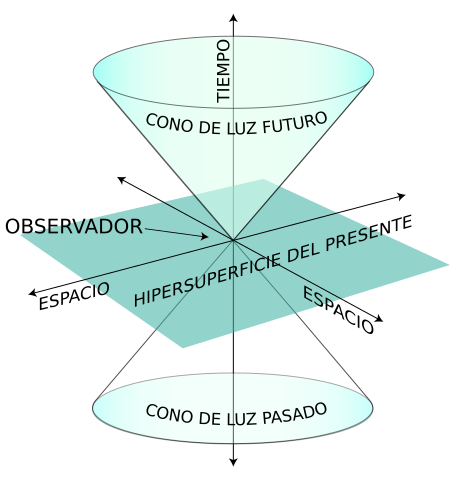
\includegraphics[width=.4\textwidth]{Fotos/470px-World_line-es.svg.png}
\caption{Un evento en un cono de luz temporal}
\end{figure}

\clearpage

\subsection{Tablas y Gráficos}
Los resultados de estas tablas fueron obtenidos con el código proporcionado para partículas con una velocidad inicial $v_0 = 2.156\cdot 10^{8}\ m/s$ y bajo la influencia de un campo magnético de $B = 0.93\ T$ 
\begin{table}[h]
\setlength{\tabcolsep}{3pt}
    \renewcommand{\arraystretch}{1.2}
    \centering
\begin{tabular}{ | c | c | c | c | c |} 
    \hline
     & \multicolumn{2}{ |c| }{Cálculo analítico} & \multicolumn{2}{ |c| }{Cálculo numérico}\\
    \hline
    Elemento & $f_a (Hz)$ & $R_a (m)$ & $f_n (Hz)$ & $R_n (m)$ \\
    \hline
    $e^-$ & $-2.6\cdot 10^{10}$ & $-1.322\cdot 10^{-3}$ & $-2.6\cdot 10^{10}$ &  $-1.322\cdot 10^{-3}$  \\
    $e^+$ & $2.6\cdot 10^{10}$ & $1.322\cdot 10^{-3}$ & $2.6\cdot 10^{10}$ & $1.322\cdot 10^{-3}$ \\
    $p^+$ & $1.418\cdot 10^{7}$ &  $2.424$ & $1.418\cdot 10^{7}$ & $2.424$ \\
    \hline
\end{tabular}
    \caption{Resultados no relativistas}
\end{table}

\begin{table}[h]
\setlength{\tabcolsep}{3pt}
    \renewcommand{\arraystretch}{1.2}
    \centering
\begin{tabular}{ | c | c | c | c | c |} 
    \hline
     & \multicolumn{2}{ |c| }{Cálculo analítico} & \multicolumn{2}{ |c| }{Cálculo numérico}\\
    \hline
    Elemento & $f_a (Hz)$ & $R_a (m)$ & $f_n (Hz)$ & $R_n (m)$ \\
    \hline
    $e^-$ & $-1.803\cdot 10^{10}$ & $-1.907\cdot 10^{-3}$ & $-1.803\cdot 10^{10}$ &  $-1.9067\cdot 10^{-3}$  \\
    $e^+$ & $1.803\cdot 10^{6}$ & $1.907\cdot 10^{-3}$ & $1.803\cdot 10^{10}$ &  $1.9067\cdot 10^{-3}$  \\
    $p^+$ & $9.834\cdot 10^{6}$ &  $3.496$ & $9.835\cdot 10^{6}$ & $3.495$ \\
    \hline
\end{tabular}
    \caption{Resultados relativistas}
\end{table}

\begin{figure}[h]
    \centering
    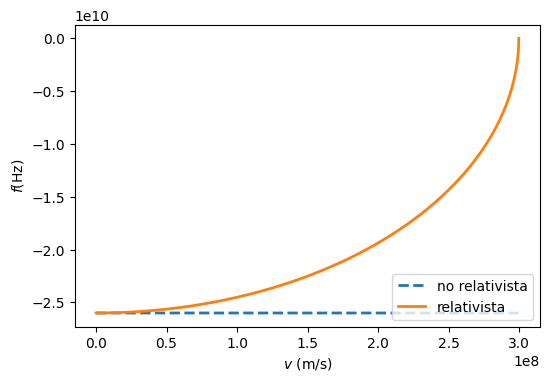
\includegraphics[width=.36\textwidth]{e-.png}
    \label{$e^-$}
    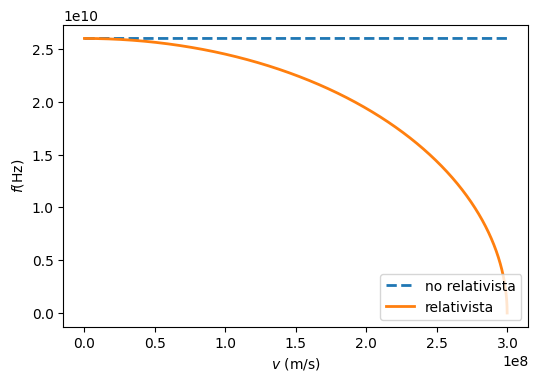
\includegraphics[width=.36\textwidth]{e+.png}
    \label{$e^+$}
    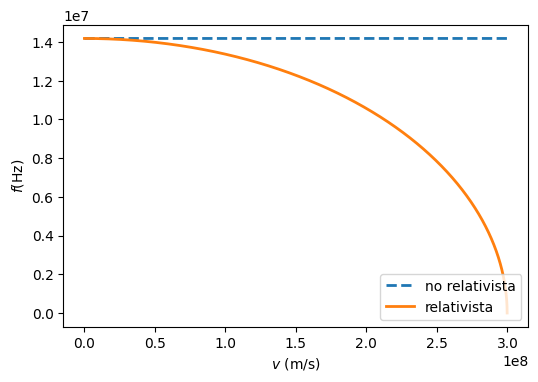
\includegraphics[width=.36\textwidth]{p+.png}
    \label{$p^+$}
    \caption{(a) e- (b) e+ (c) p+
    }
    \label{fig:foobar}
\end{figure}

\clearpage

\section{Ciclotrón}
\hfill
\subsection{Introducción}
El método directo de acelerar iones utilizando la diferencia de potencial presentaba grandes dificultades experimentales asociados a los campos eléctricos intensos. El ciclotrón evita estas dificultades por medio de la aceleración múltiple de los iones hasta alcanzar elevadas velocidades sin el empleo de altos voltajes.\\

Las partículas cargadas, al principio en reposo y situadas en el origen del dispositivo, son aceleradas por medio de la acción de un campo eléctrico variable en el medio de las 2 zonas a modo de D. En todo el trayecto de las partículas hay un campo magnético perpendicular que les crea un desviamiento circular, cuyo radio es dependiente de la velocidad de las partículas. El campo eléctrico debería cambiar de forma periódica a fin de que en cada paso por la zona de en medio de las 'Ds' se haga una ganancia de velocidad.\\
\hfill
\begin{figure}[h]
\centering
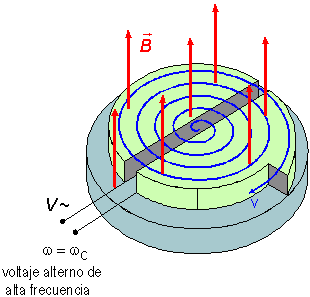
\includegraphics[width=.4\textwidth]{ciclotron (1).png}
\end{figure}
\hfill

Su energía cinética final será tantas veces mayor que la que corresponde al voltaje aplicado a los electrodos multiplicado por el número de veces que el ion ha pasado por la región intermedia entre las 'Ds'.

\subsection{Resultados y Gráficas}
\hfill\\
Todos los resultados calculados en esta tabla fueron obtenidos para un ciclotrón con una diferencia de potencial entre sus placas de $dV= 4390\ V$, valor obtenido aleatoriamente. \\

\begin{table}[h]
\setlength{\tabcolsep}{3pt}
    \renewcommand{\arraystretch}{1.3}
    \centering
    \centering
\begin{tabular}{ | c | c | c | c | c |} 
    \hline
     & \multicolumn{4}{ |c| }{Resultados} \\
    \hline
    Partícula & f (Hz) & $\frac{T}{2}(s)$ & $\Delta{E_c}(J)$ & v (m/s) \\
    \hline
    $H^+$ &  6.099E+06 Hz & 1.640E-07 s & 7.024E-16 J & 9.172E+05 m/s  \\
    $2H^+$ & 3.068E+06 Hz & 3.259E-07 s & 7.024E-16 J & 6.505E+05 m/s \\
    $3H^+$ & 2.045E+06 Hz & 4.889E-07 s & 7.024E-16 J & 5.311E+05 m/s \\
    $4H^{++}$ & 3.046E+06 Hz & 3.283E-07 s & 9.237E-16 J & 7.125E+05 m/s \\

    \hline
\end{tabular}
    \caption{Tabla de los datos obtenidos del protón, deuterio y tritio}
    \label{tabla-ciclo}
\end{table}


\clearpage

\centering
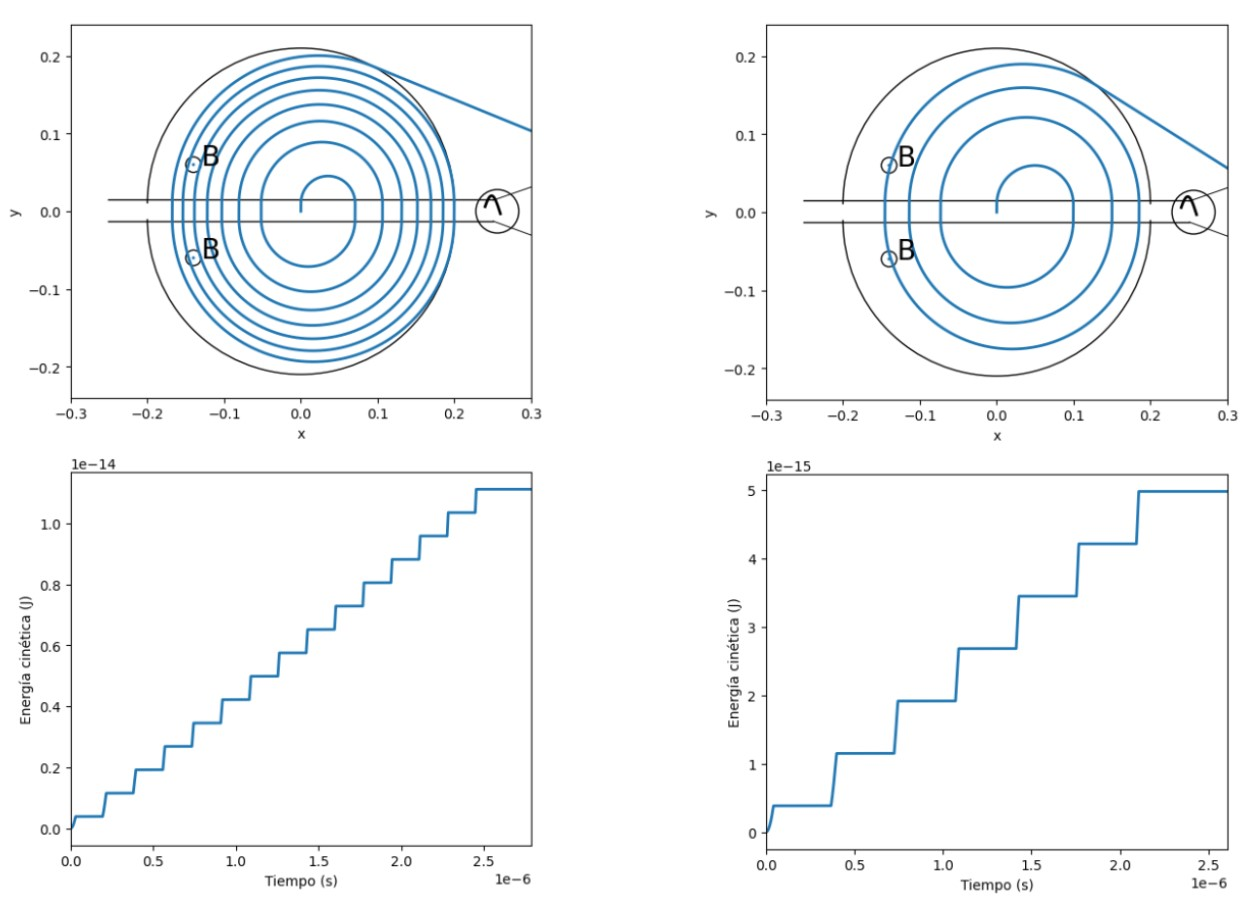
\includegraphics[width=.95\textwidth]{lucas1.jpg}\\
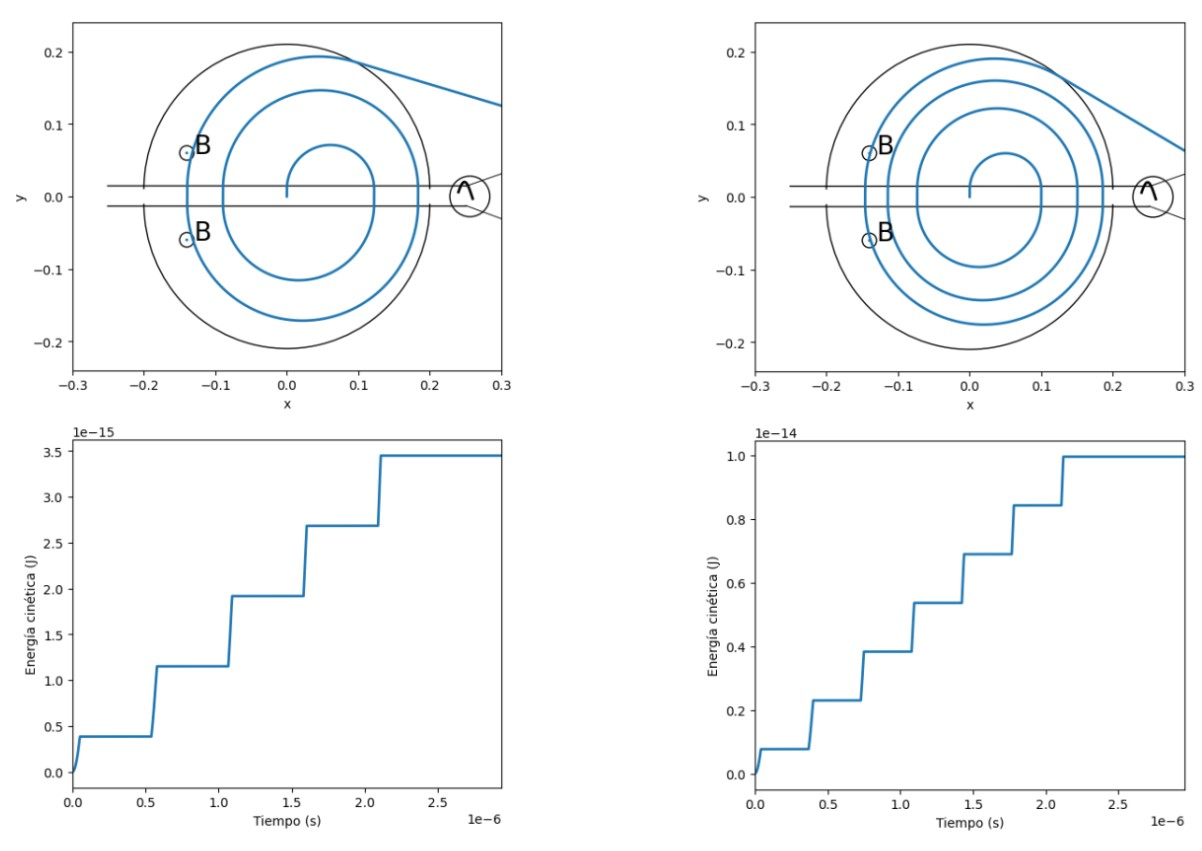
\includegraphics[width=.95\textwidth]{lucas2.jpg}

\clearpage

\section{Conclusiones}
\justify
\subsection{Espectrómetro}
\noindent Efectivamente los resultados obtenidos numéricamente
coinciden con los resultados esperados, los calculados analíticamente de forma previa. El error es del orden de $10^{-9}$ para el tiempo y de $10^{-6}$ para la distancia. La coincidencia entre resultados numéricos y analíticos se repite en todos los isótopos comprobados. \\ \\
Además, gracias a las gráficas podemos determinar que a mayor masa, los isótopos recorrerán una mayor distancia, que también se cumple para todos los grupos de isótopos comprobados. \\ \\Cabe destacar como en el caso del calcio, uno de los isótopos tiene una carga significativamente mayor al resto y podemos observar en su gráfica cómo la distancia recorrida es significativamente mayor.
\vspace{0.5cm}
\subsection{Relatividad}
\noindent A modo de conclusión de este apartado podemos ver como los resultados analíticos coinciden en su totalidad con los resultados obtenidos numéricamente por nuestro código. \\ \\En segundo lugar compararemos los resultados relativistas con los no relativistas. En los relativistas, las frecuencias son menores, pero en cambio los radios de giro son mayores que su antagonista no relativista. Esto se debe a que la masa relativista tiene una gran influencia en el radio de giro. Al cambiar este pero no variar la velocidad de la partícula, la frecuencia baja, ya que logrará dar menos vueltas.
\vspace{0.5cm}
\subsection{Ciclotrón}
\noindent De los resultados, deducimos que las muestras con distintas masas y cargas, se comportarán de diferente manera dentro del ciclotrón. En la tabla de resultados, observamos como para el protón, el núcleo de deuterio y el de tritio (partículas con la misma carga y
diferente masa) la variación de energía cinética es la misma, ya que la energía cinética dependerá de la carga y no de la masa.\\ \\Vemos también como la velocidad de salida del aparato también es igual, y destacamos como a mayor cantidad de neutrones en la partícula (es decir, mayor masa) la velocidad al salir del ciclotrón será menor. Al tener más masa, mayor será el radio de giro, y por lo tanto, la partícula saldrá antes del ciclotrón, evitando que la partícula adquiera más energía cinética. (La diferencia de radio se hace notable en las representaciones gráficas).\\ \\En los gráficos observamos las diversas trayectorias que han seguido las partículas. A su vez se muestra el aumento de la energía cinética a su paso por el ciclotrón. Todas las variaciones de la energía cinética siguen un patrón similar, ya que todas las partículas adquieren energía cinética de la misma manera, es decir, solo adquirirán energía cinética (velocidad) cuando pasen entre las D’s (lugar donde existe un campo eléctrico). Es por ello, que la velocidad se va ganando de forma escalonada y no de forma lineal.\\ \\Para acabar, destacar que si variamos la frecuencia angular con la que oscila el voltaje entre las D’s en un 50\%, para que el ciclotrón funcione y no nos de resultados erróneos, debemos cambiar el tipo de frecuencia del generador de campo eléctrico. La frecuencia debe variar de una función cuadrada a una función cosenoidal. Una vez cambiadas las frecuencias, el ciclotrón se comportará de la misma forma
que en los casos mencionados anteriormente.

\clearpage
\section{Códigos}
Espectrómetro: \href{https://drive.google.com/file/d/1POTN37wFfRKkrrgz9a6X_jpjA8OC4kvs/view?usp=sharing}{Código espectrómetro de masas} 

\vspace{.3cm}
Relatividad: \href{https://colab.research.google.com/drive/10xDyIfiMp-wUHr9GvP8pyn52G2KDsUSn?usp=sharing}{Código para la relatividad} 

\vspace{.3cm}

Ciclotrón: \href{https://colab.research.google.com/drive/1RwmH6mzifx4BxK_OHAIchd6x02lqrsi5?usp=sharing}{Código del ciclotrón} 

\end{document}